\documentclass[12pt,a4paper,UTF8]{article}
\usepackage{ctex} % Chinese support
\usepackage{graphicx} % Insert images
\usepackage{subfigure}
\usepackage{float}
\usepackage{listings} % Print source code
\usepackage{color} % Color support
\usepackage{booktabs} % Professional table support
\usepackage{pdflscape} % Landscape pages support in PDF
\usepackage{hyperref} % Hypertext links support for cross-referencing
\usepackage{amsmath,mathtools}
\usepackage{ulem} % strikethrough

% Customize hyperref format (it's set to no special format here)
\hypersetup{hidelinks}

% Declare directories to search for graphics files for graphicx
\graphicspath{{figures/}}

% Define source code style for listings
\lstdefinestyle{verilog-style}{
	language=Verilog,
	basicstyle=\ttfamily\footnotesize,
	keywordstyle=\bfseries\color[rgb]{0, 0, 1},
	identifierstyle=\color[rgb]{0.5, 0.3, 0.1},
	stringstyle=\color[rgb]{0.6, 0.1, 0.1},
	commentstyle=\itshape\color[rgb]{0.05, 0.5, 0.05},
	backgroundcolor=\color[gray]{0.95},
	numbers=left,
	numbersep=5pt,
	numberstyle=\color[gray]{0.6},
	breaklines=true
}

\newcommand{\reporttitle}[2]{
  \LARGE\textsf{#1}\quad\underline{\makebox[12em]{#2}}
}

\newcommand{\reportinfo}[2]{
  \large\makebox[4em]{\textsf{#1}}\quad\underline{\makebox[18em]{#2}}
}

\begin{document}
\begin{titlepage}
  \centering
  \vspace*{\fill}
  {\Huge\textsf{数字电路与数字系统实验}} \\ [100pt]
  \reportinfo{实验名称}{exp04 触发器和锁存器} \\ [10pt]
  \reportinfo{院系}{计算机科学与技术系} \\ [10pt]
  \reportinfo{学生姓名}{} \\ [10pt]
  \reportinfo{学号}{} \\ [10pt]
  \reportinfo{班级}{数字电路与数字系统实验1班} \\ [10pt]
  \reportinfo{邮箱}{} \\ [10pt]
  \reportinfo{实验时间}{2020 年 9 月 23 日} \\ [10pt]
  \vspace*{\fill}
\end{titlepage}
\tableofcontents
\newpage

\section{实验目的}
\begin{itemize}
  \item 复习锁存器和触发器的原理
  \item 回顾时序电路的知识
  \item 学习Verilog中的时序电路设计,以及
        阻塞赋值语句和非阻塞赋值语句的区别
  \item 学习Verilog中模块实例化的方法
\end{itemize}

\section{实验原理}
\begin{description}
  \item[锁存器] 锁存器的通过激励输入的电平来控制
        元件的状态,数据有效滞后于使能信号有效
  \item[触发器] 触发器具有时钟控制信号,该信号
        的边沿向触发器发出命令,触发器根据激励
        信号改变状态。在多触发器的电路中,时钟信号
        可以使所有的触发器同步的改变状态。
  \item[阻塞赋值语句] 立即计算赋值语句右边表达式的值,
        并把它赋给语句左边的变量
  \item[非阻塞赋值语句] 立即计算赋值语句右边表达式的值,
        但是要等到整个always块执行完毕后,经过一个无穷小
        的延迟才完成赋值
  \item[同步清零] 在时钟脉冲有效时,根据清零信号进行清零
  \item[异步清零] 清零信号有效时立即清零
\end{description}

\section{实验环境/器材}
\begin{itemize}
  \item Quartus编辑器和DE10-Standard开发平台
  \item FPGA开发板
\end{itemize}

\section{程序代码+实验过程+测试方法}
\subsection{实验4.3.1 阻塞与非阻塞}
实验4.3.1即把实验4.2中给出代码在自己的电脑上实现一下,
代码和RTL视图都和4.2里的一毛一样。为了证明自己确确实实
认认真真地照抄了一遍,那就贴一下RTL图片意思一下:
\begin{figure}[H]
  \centering
  \subfigure[阻塞赋值语句设计的触发器]{
    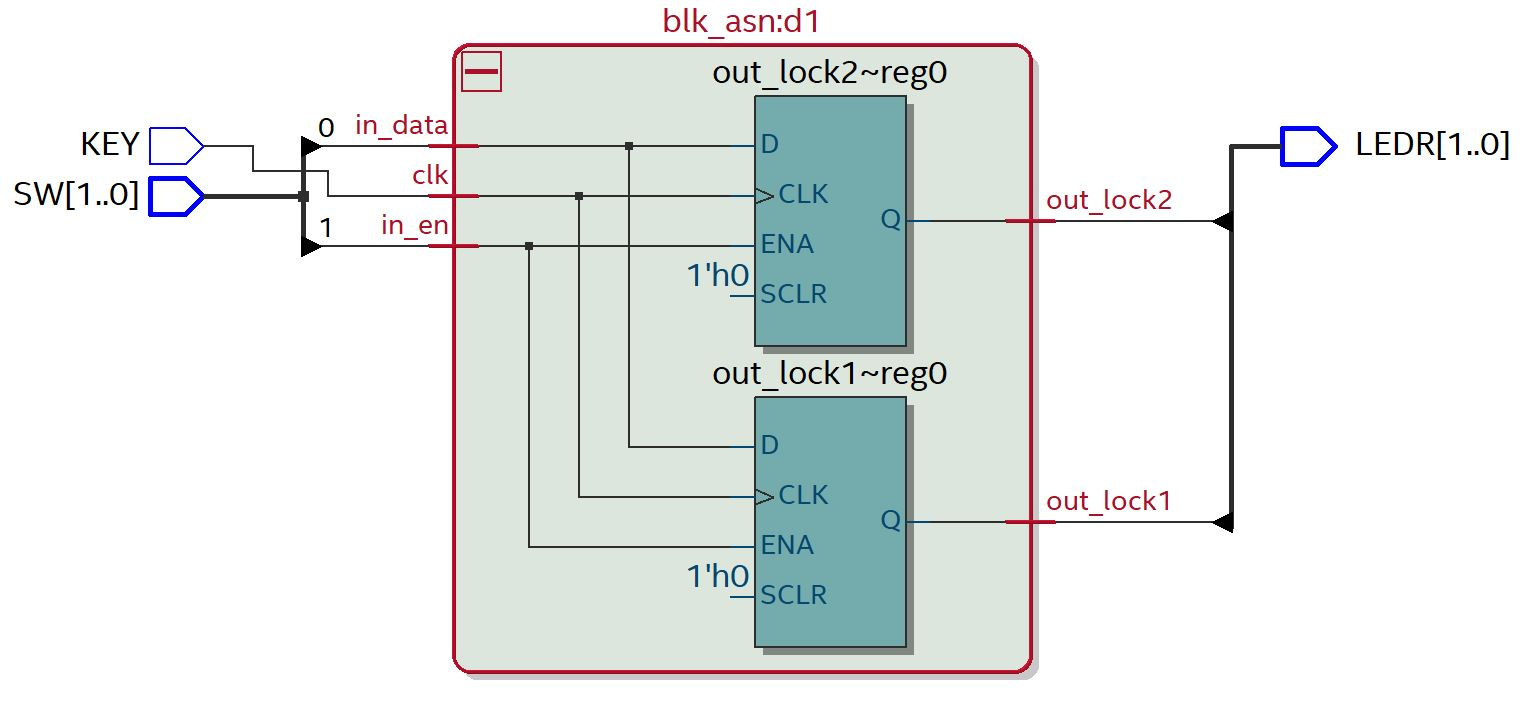
\includegraphics[width=0.45\textwidth]{rtl_blk_asn.JPG}
  }
  \subfigure[非阻塞赋值语句设计的触发器]{
    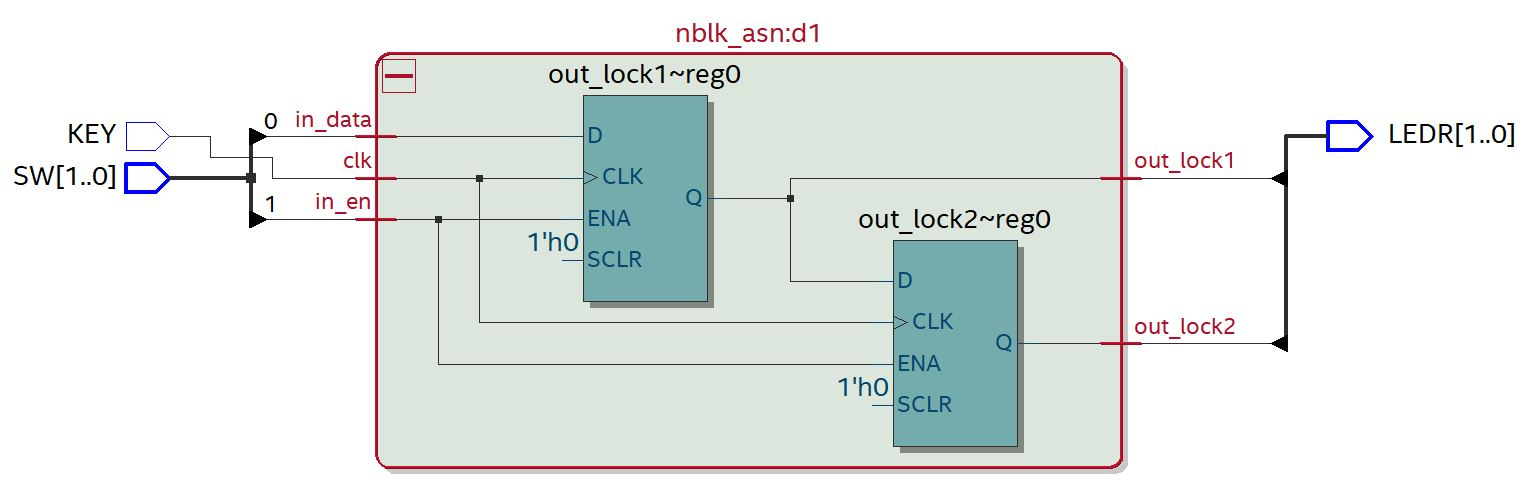
\includegraphics[width=0.45\textwidth]{rtl_nblk_asn.JPG}
  }
  \caption{RTL视图}
  \label{RTL}
\end{figure}

这里主要描述一下我写的测试文件。因为一开始照搬实验4.1里
代码4-4时出了一点小bug,所以我采用了另一种方式------
多个always程序块来编写测试文件(其实主要原因是代码4-4不优雅)。
先看测试代码:
\begin{lstlisting}[style=verilog-style]
initial
begin
	KEY = 0; SW = 2'b0;
	# 300;
	$stop;
end

always begin
	#0.2 KEY = 1; #10; 
	KEY = 0; #9.8;
end                                                    

always begin
	#2 SW[1] = ~SW[1]; #58;
end

always begin
	#3 SW[0] = ~SW[0]; #12;
end 
\end{lstlisting}

KEY对应的是FPGA开发板上的按钮,用来模拟时钟信号。
按下按钮是低电平(KEY=0),松开是高电平(KEY=1)。
SW[1]是使能信号,SW[0]是输入信号D。

在initial程序块中,先给KEY和SW赋上初始值,然后等待
300个时钟周期。在这段时间里,三个always块同时运行,
时钟信号每10个时钟周期改变一下,使能信号60,输入信号15。
300个时钟周期之后在initial块中执行\$stop指令,停止测试。

为了波形可读性,时钟信号先经过一个小的偏移再开始上升沿。
其他两个信号也都有所偏移。仿真运行结果如下:
\begin{figure}[H]
  \centering
  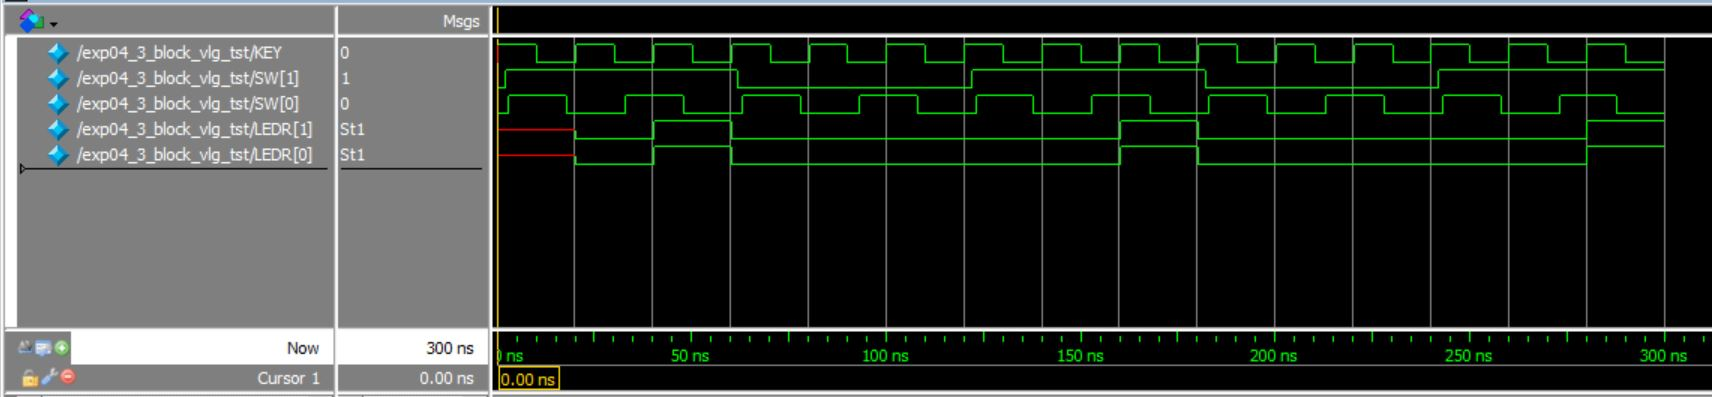
\includegraphics[width=1\textwidth]{sim_blk_asn.JPG}
  \caption{阻塞赋值语句触发器的仿真图}
  \label{sim_blk}
\end{figure}

\begin{figure}[H]
  \centering
  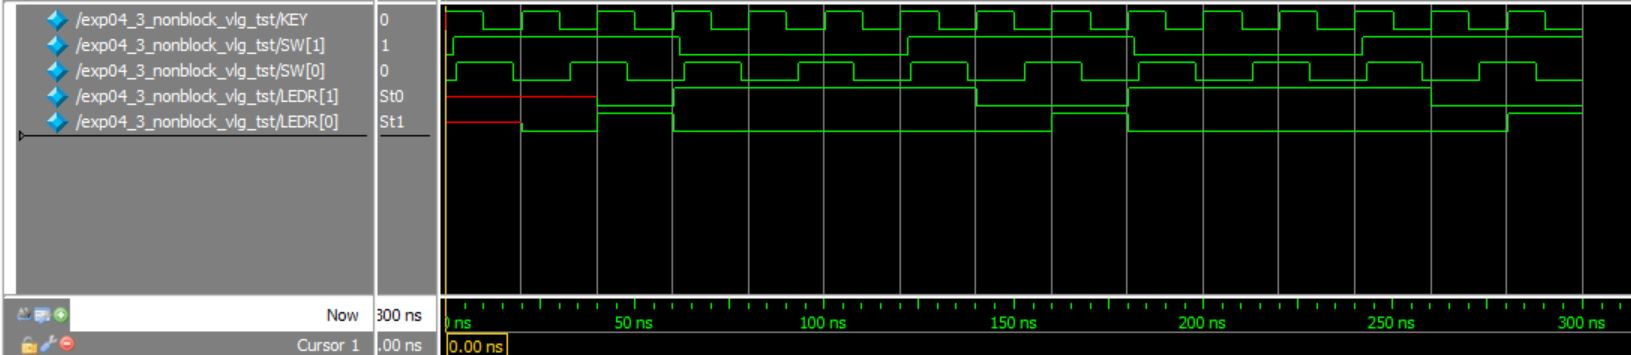
\includegraphics[width=1\textwidth]{sim_nblk_asn.JPG}
  \caption{非阻塞赋值语句触发器的仿真图}
  \label{sim_nblk}
\end{figure}

\subsection{实验4.3.2 part1同步清零和异步清零}
同步清零和异步清零的区别已经在``实验原理''条目中叙述
过了,在此不做赘述。这里简单介绍一下分配的引脚:KEY是
时钟信号,SW[1]是清零信号,SW[0]是输入信号,LEDR是输出
信号。下面直接上代码、RTL和仿真结果:

\subsubsection{同步清零}
\begin{lstlisting}[style=verilog-style]
always @ (posedge CLK)
  if (CLR) Q <= 0;
  else Q <= D;
\end{lstlisting}
\begin{figure}[H]
  \centering
  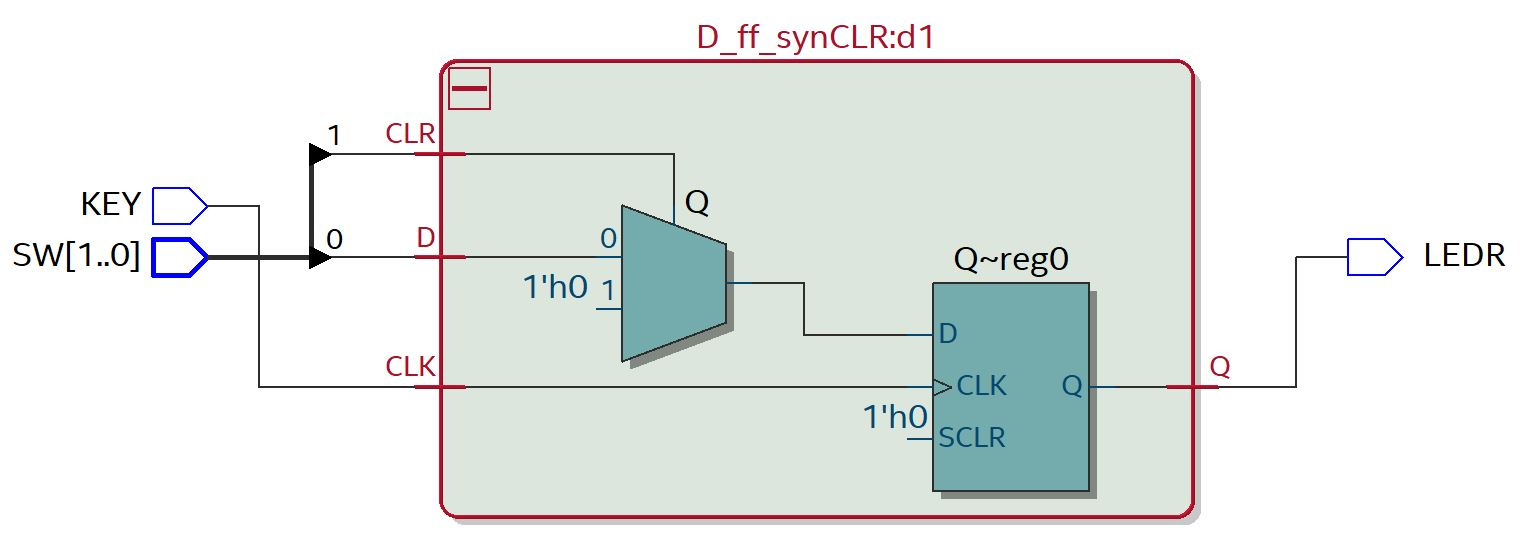
\includegraphics[width=1\textwidth]{rtl_synCLR.JPG}
  \caption{同步清零触发器的RTL视图}
  \label{rtl_synCLR}
\end{figure}
\begin{figure}[H]
  \centering
  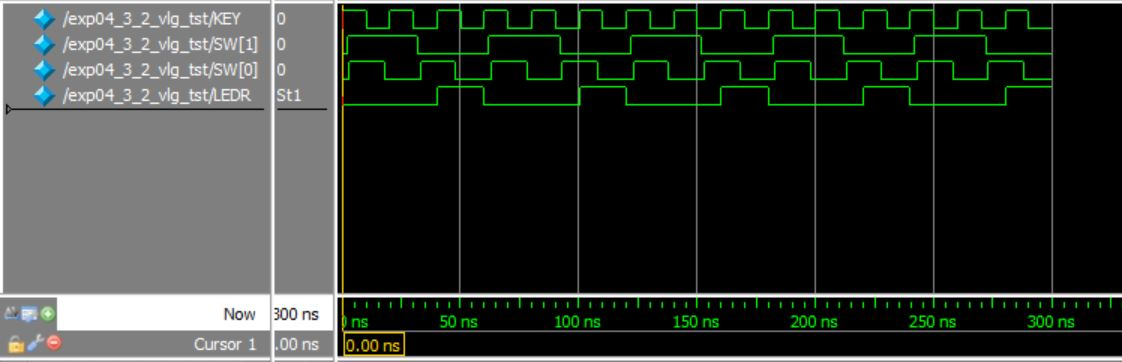
\includegraphics[width=1\textwidth]{sim_synCLR.JPG}
  \caption{同步清零触发器的仿真结果}
  \label{sim_synCLR}
\end{figure}
\hspace*{\fill}\\

\subsubsection{异步清零}
\begin{lstlisting}[style=verilog-style]
always @ (posedge CLK or posedge CLR)
	if (CLR) Q <= 0;
	else Q <= D;
\end{lstlisting}
\begin{figure}[H]
  \centering
  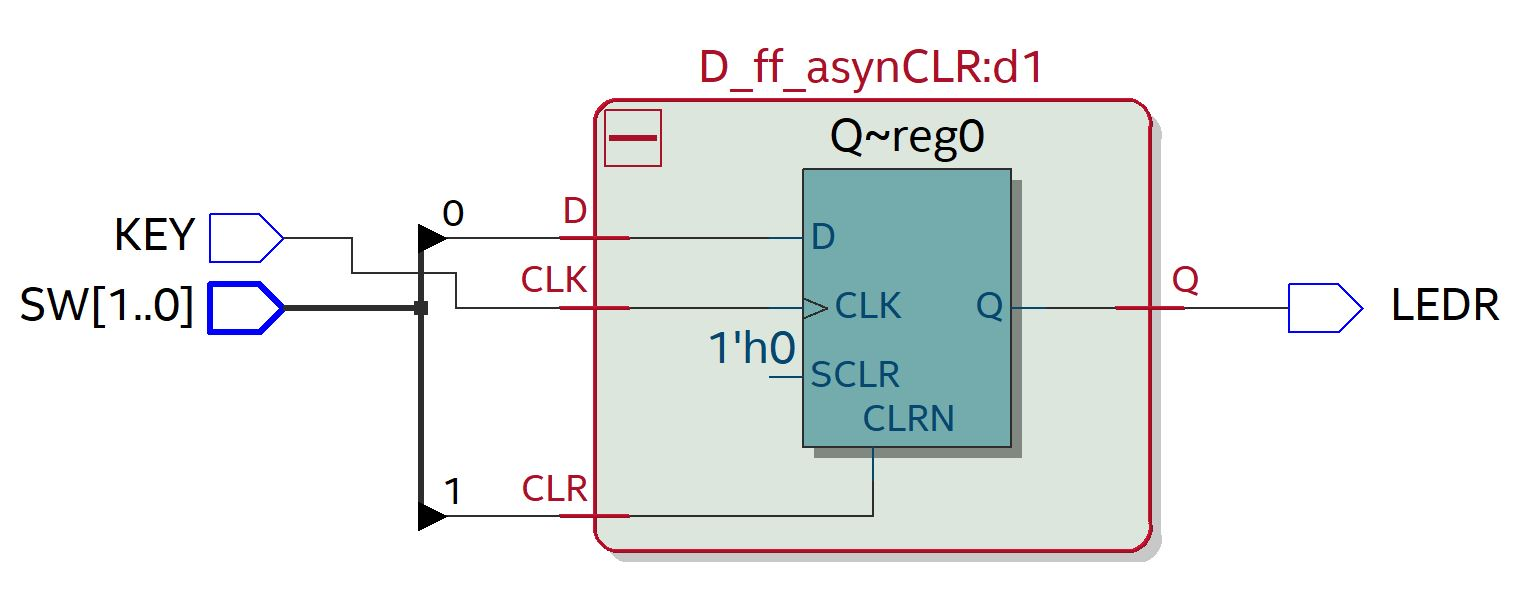
\includegraphics[width=1\textwidth]{rtl_asynCLR.JPG}
  \caption{同步清零触发器的RTL视图}
  \label{rtl_asynCLR}
\end{figure}
\begin{figure}[H]
  \centering
  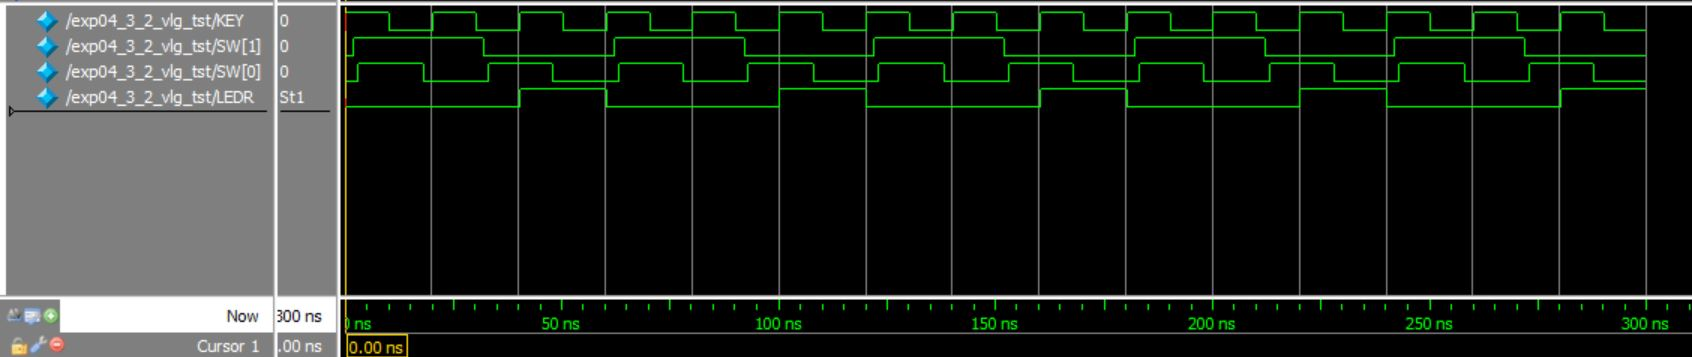
\includegraphics[width=1\textwidth]{sim_asynCLR.JPG}
  \caption{异步清零触发器的仿真结果}
  \label{sim_asynCLR}
\end{figure}

\subsection{实验4.3.2 part2顶层模块与仿真分析}
在顶层模块中实例化两个子模块,重新分配引脚如下:KEY是
时钟信号,SW[2]是两个触发器共用的清零信号,SW[0]和LEDR[0]
是同步清零触发器的输入信号和输出信号,SW[1]和LEDR[1]是
异步清零触发器的输入信号和输出信号。
\begin{figure}[H]
  \centering
  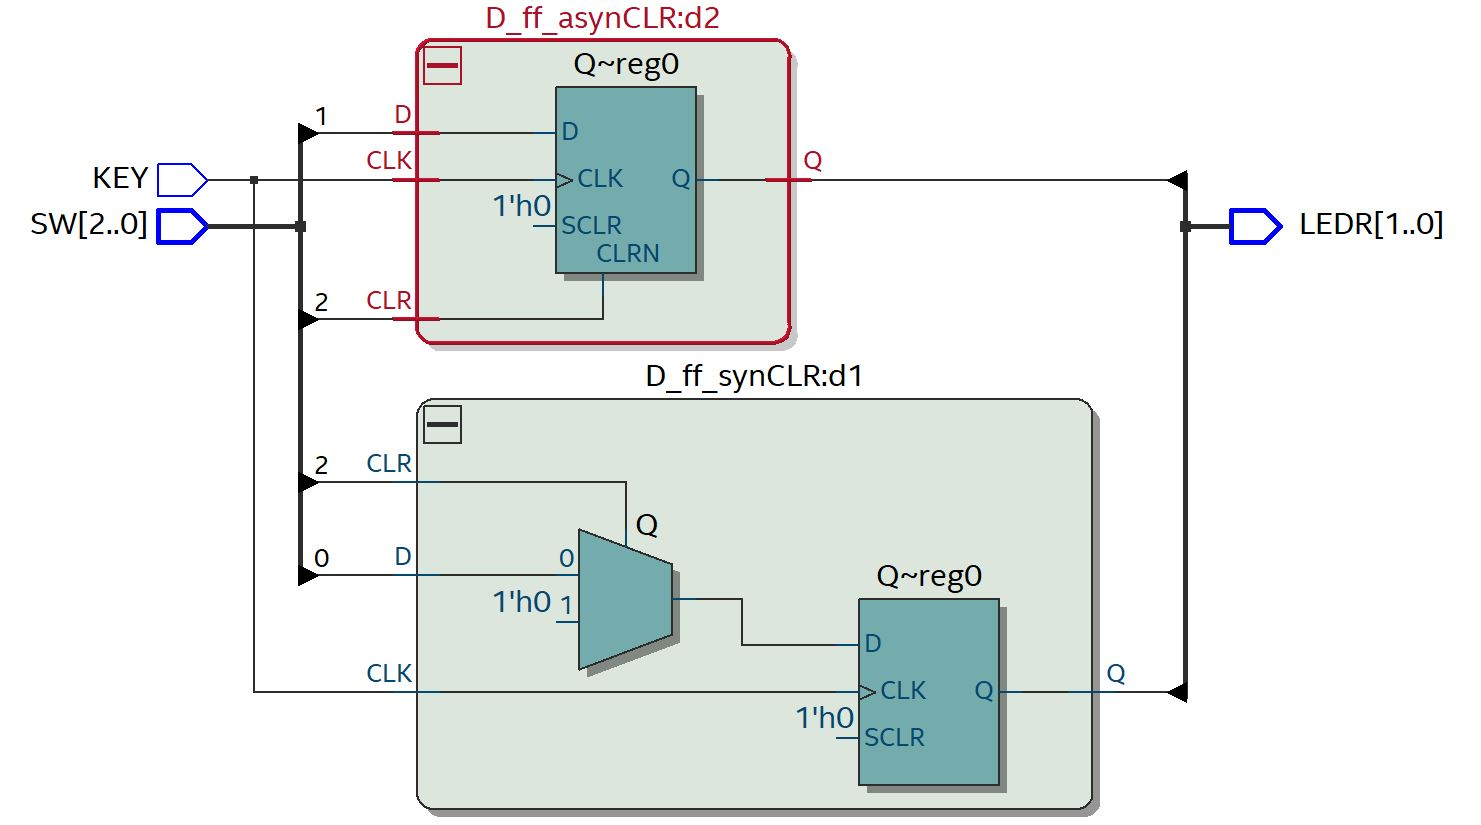
\includegraphics[width=1\textwidth]{rtl_top.JPG}
  \caption{RTL视图}
  \label{rtl_top}
\end{figure}
\begin{figure}[H]
  \centering
  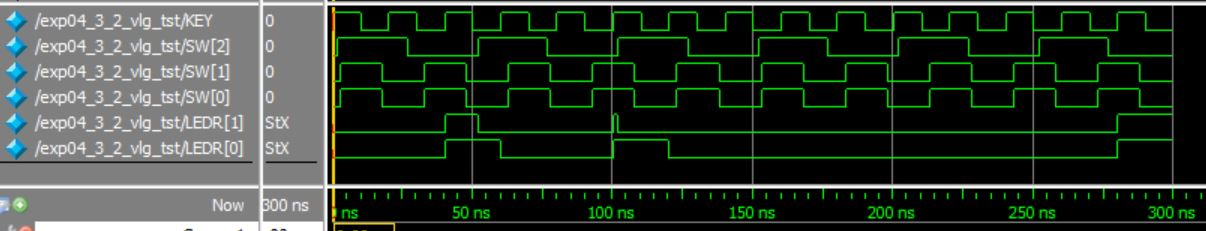
\includegraphics[width=1\textwidth]{sim_top.JPG}
  \caption{仿真结果}
  \label{sim_top}
\end{figure}

从仿真结果不难看出,当清零信号产生时,异步清零的触发器
输出立刻清零,而同步清零的触发器会只会在时钟信号上升沿时
根据清零信号清零。

\section{实验结果}
成功。

\sout{为了使此条目看起来不那么敷衍了事,所以贴一下FPGA实验图:}
\begin{figure}[H]
  \centering
  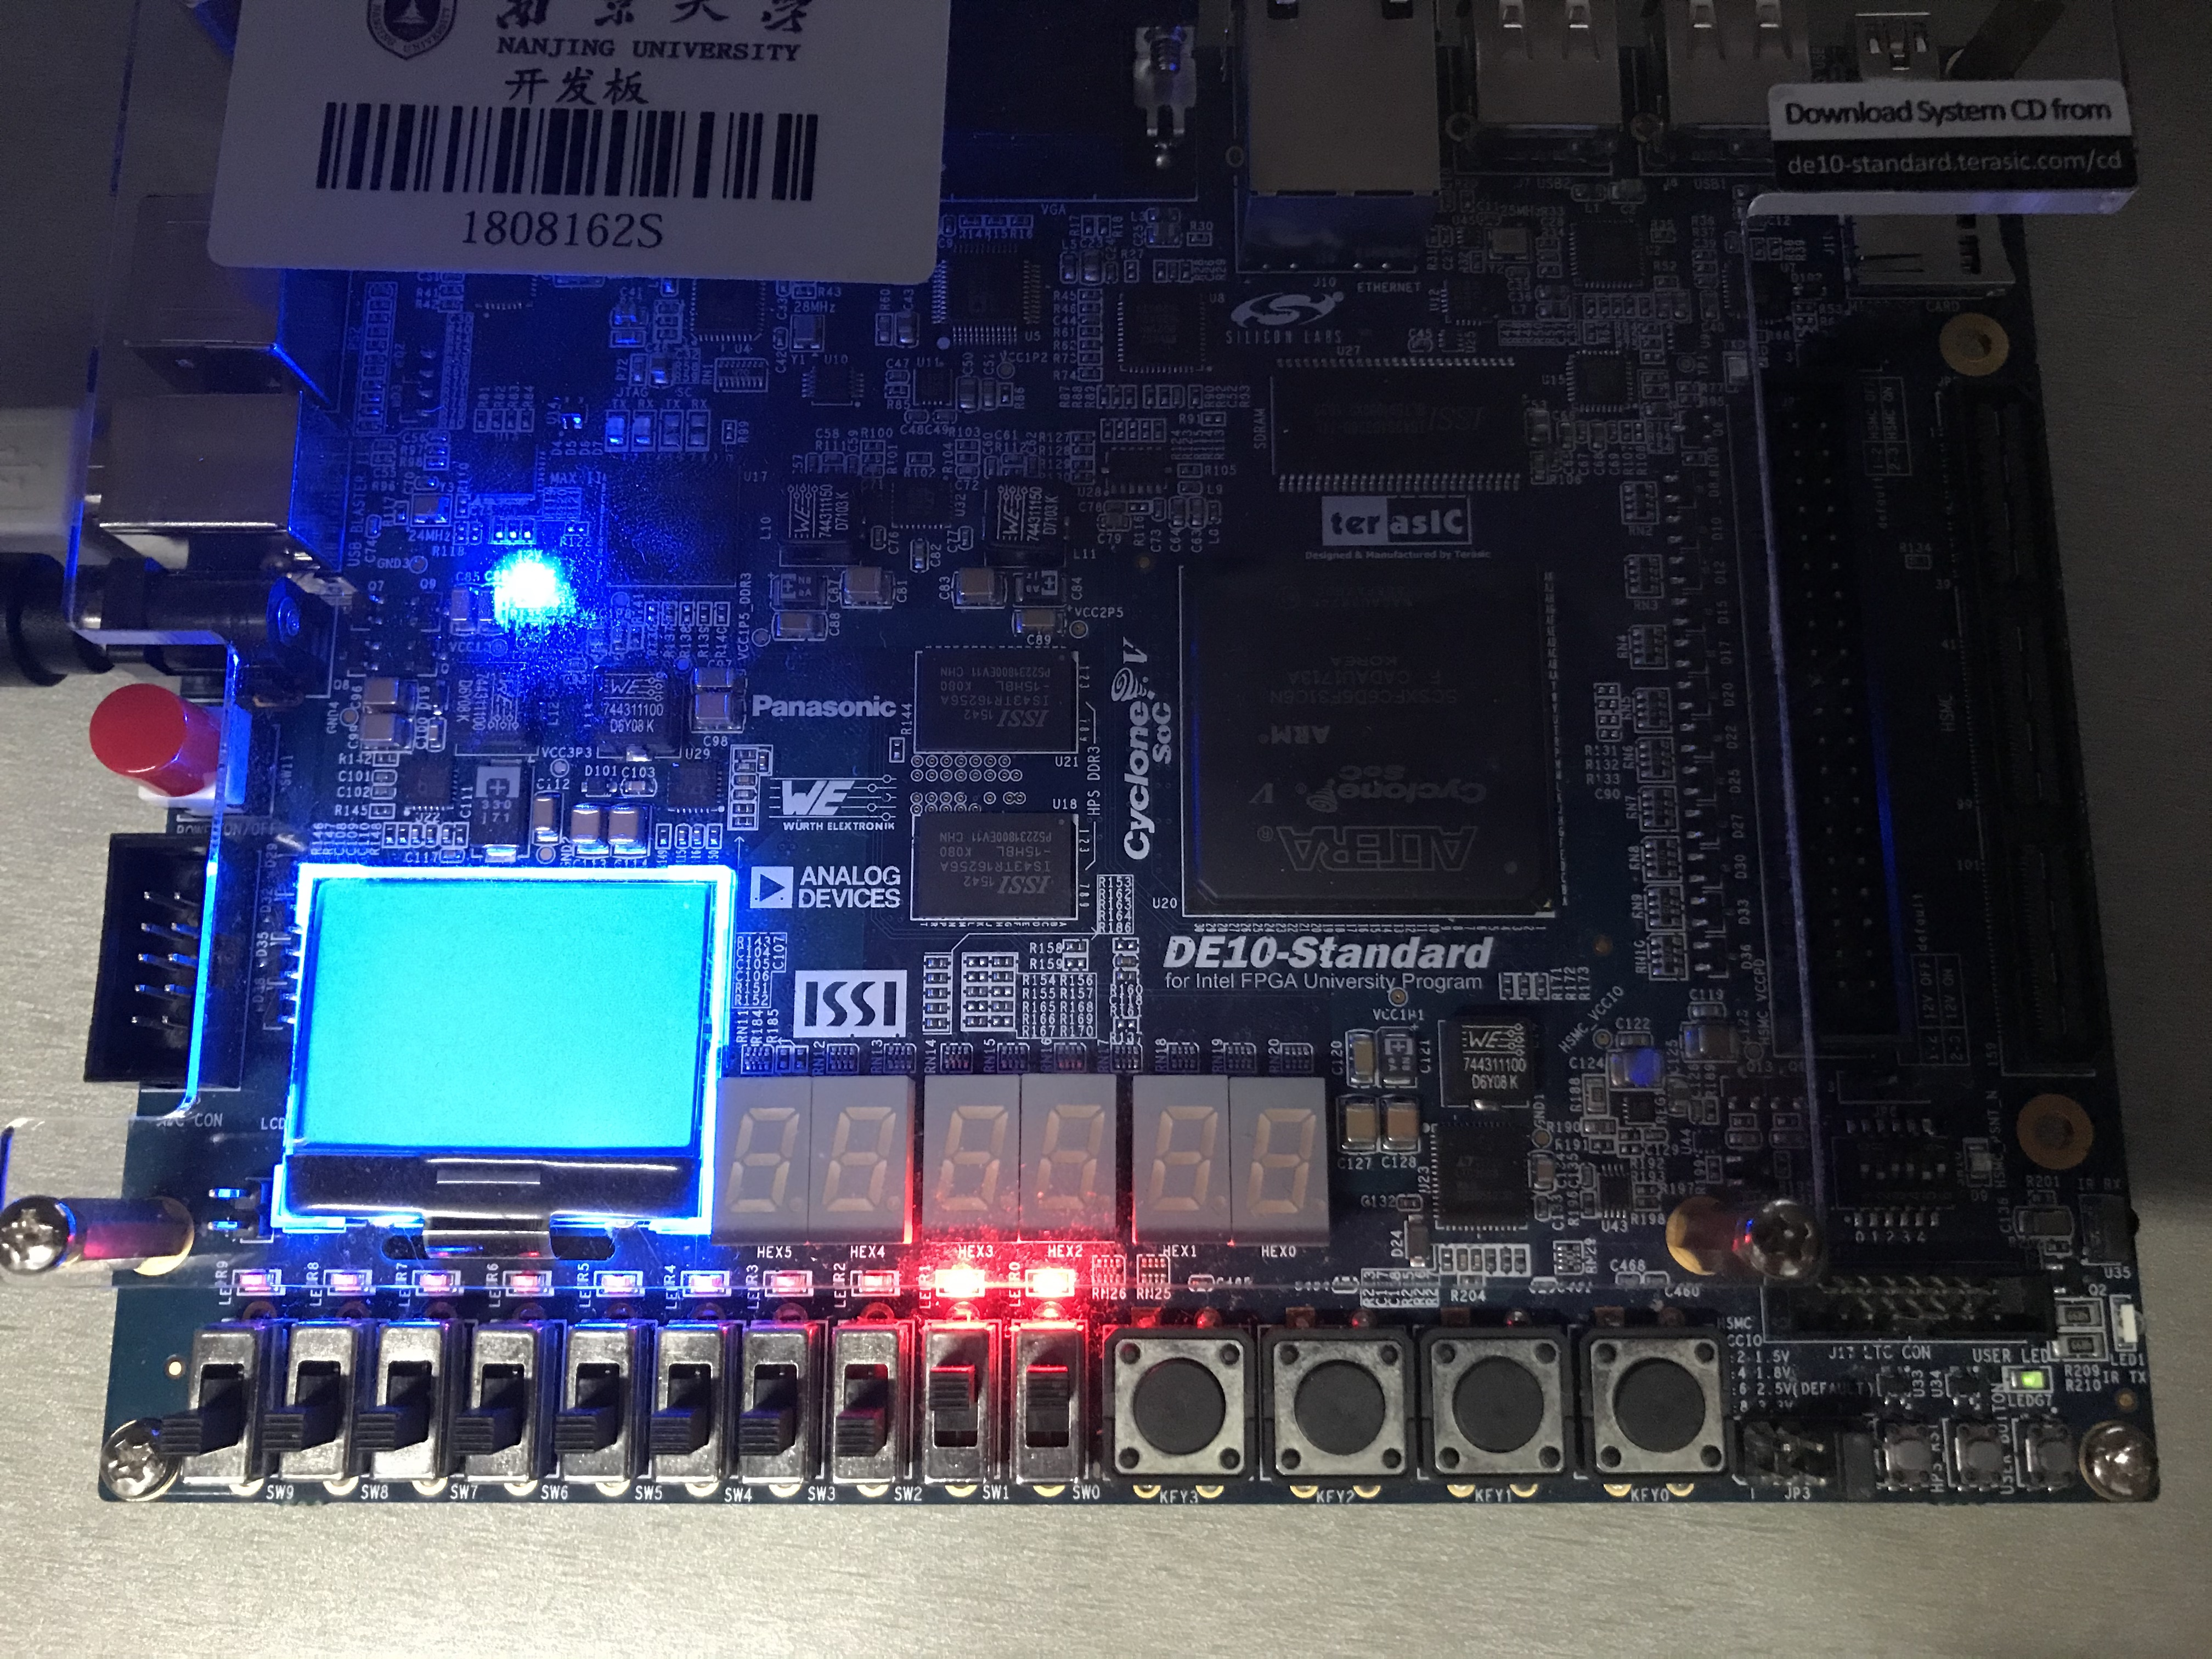
\includegraphics[width=1\textwidth]{FPGA_top.JPG}
  \caption{实验4.3.2下载运行结果}
  \label{FPGA_top}
\end{figure}

\section{遇到的问题及解决办法}
\begin{itemize}
  \item 照着实验4.1里的代码4-4写测试文件,
        把clk=$\sim$clk中的取反号写成了负号。
        clk初始值赋的是0,然后不断取反还是是0。
        找了一晚上才找到这个bug(T\_T)
  \item 用DE10\_Standard\_SystemBuilder创建工程
        会自动生成顶层文件。这时候如果自己调整顶层
        文件,那么在仿真运行的时候就会出现亿点点问题。
        所以当工程自动设置好顶层文件之后,就不要
        乱动顶层文件了。
  \item 用DE10\_Standard\_SystemBuilder创建工程,
        会自动分配引脚并生成主模块的输入参数。如果有的
        器件生成时给了多个但我们只需要用一个
        (如switch和button),那么也需要写
        ``input [0:0] XXX''。其中``[0:0]''不能省略,
        否则Verilog会认为这些器件全部都使用。也就是说,
        当我们把参数XXX传递给子模块时(这里我们写的是XXX
        而不是XXX[0]),如果我们在前面写了``input [0:0] XXX'',
        那么我们传递的就是XXX[0];如果我们漏写了``[0:0]'',
        那么我们传递的是所有的XXX而非只有一个XXX,继而会
        产生一些意想不到的错误。
\end{itemize}

\section{得到的启示}
\begin{itemize}
  \item 可以在模块文件中给模块输出的寄存器
        赋初始值,那么在仿真运行的波形图中,
        输出端就不会出现不确定值(其是并没有
        必要这样做,虽然没有红线看起来舒服
        一点,但是没有红线有悖于实验现象)
        \begin{figure}[H]
          \centering
          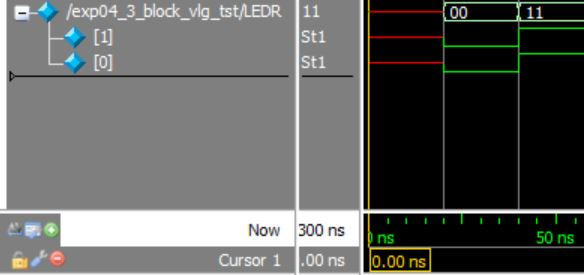
\includegraphics[width=0.8\textwidth]{bugfix1.JPG}
          \caption{输出端的不确定值}
          \label{bugfix1}
        \end{figure}
  \item always程序块内部是顺序执行的,多个always程序块是并发执行的
\end{itemize}


\section{意见和建议}
\begin{itemize}
  \item 实验4.2第三段``always''拼写错了(\^{}\_\^{})
\end{itemize}

\end{document}